%% General discussion

The original hypothesis of this research was that "\textit{Individual and population level air pollutant exposure can be estimated using time-activity surveys, GIS and routing tools, and then coupled with high resolution spatio-temporal air quality models to facilitate a greater understanding of the health impacts of air pollution and how public health risks can be reduced}". Overall, this research has proved this hypothesis through the creation of a tool that allows scientists to examine individual-level and group exposure to ranges of pollutants in a range of microenvironments. Chapters \ref{chap:the_ltdsx} and \ref{chap:the_lhem}, which were the main chapters centred around the creation of the tool, have been published as \cite{Smith2016} (the model development and use), and then subsequently used by \cite{Tonne2018} to examine socioeconomic and ethnic inequalities in exposure to poor air quality. Chapter \ref{chap:monitoring_on_underground}, refining the exposure estimates for users of the London Underground after this microenvironment was found to be so important to Londoners exposure, is in the process of being written-up as an academic paper and will provide an open-source dataset ('TubeAir') for calculating exposure of London Underground users within other studies, or as a stand-alone policy tool. Chapter \ref{chap:evaluating_dynamic_exposure_models}, on how to evaluate exposure models of this kind, diverted away from the main hypothesis of the research, but during chapters \ref{chap:the_ltdsx}, \ref{chap:the_lhem} and \ref{chap:monitoring_on_underground} the reliability and representativeness of the results became something of interest (and importance) to consider, and so this seemed necessary.\\

%% Discussion on LTDS-X
In more detail, Chapter \ref{chap:the_ltdsx} demonstrated how a dataset that was originally purposed for assessing transport demand could be adapted, processed and re-purposed to create the LTDS-X, a high resolution spatial and temporal time-activity dataset, including demographics, that is representative of the daily movements of the population of London. The main limitations with using this dataset as an input to the exposure modelling, were that the data were London-centric, and 'porting' this method to another city or country would require a similar or replacement dataset. Although whilst undertaking this research other datasets have been investigated and considered as replacements, for example in the 2011 UK Census, a new question of 'workplace zones' was asked of the population, and research by Dr Reis (Centre for Ecology and Hydrology, UK) is using the responses as a way to model population-level movement for exposure modelling. Using this as a basis, travel exposure from workplace zone to workplace zone by each mode of transport could be simulated and the exposure calculated, and then an indoor exposure module 'plugged-in' to create a UK-wide exposure model. The spatial detail would not be as high as the LTDS-X and LHEM, but the coverage would be much larger. Given Census' are common in many countries around the world, this could be replicated in other places given time.

It is worth noting that whilst this dataset was specifically re-purposed for use as an input to air quality exposure modelling, it could similarly be used for exposure to other things such as perhaps ultra-violet light and risks of skin-cancer, or to estimate where the population are drinking water and therefore links between poor quality water and health.

Away from exposure the dataset has been useful in other areas of work that the Environmental Research Group is involved in. In 2012 it was used to look at the number of cross-Borough car trips being undertaken as part of the London Atmospheric Emissions Inventory (LAEI), and in 2018 was used to identify whether active travel has increased or decreased in the London Borough of Waltham Forest as part of a contract piece of work.\\

%% Discussion on dynamic exposure
In Chapter \ref{chap:the_lhem}, having built the LTDS-X, this was combined with CMAQ-UK and microenvironmental modelling methods to quantify at unprecedented detail the exposure of the London population to poor air quality. The size, detail and possibilities for future research of this model were demonstrated by focusing on exposure missclassification, and this work was published in \cite{Smith2016} (which has 13 citations as of May 2018). The applications for this model are already being taken forward in other exposure studies, including the CLUE II led by Imperial College London looking at the air quality and noise exposure of children in London, and the COPE (Characterisation of COPD Exacerbations using Environmental Exposure Modelling) study led by King's College London. As was highlighted in the Chapter, it is our hope that this type of tool can increasingly be used for policy applications by the likes of TfL and London Boroughs to better understand the effects of policy interventions on exposure. Indeed, Waltham Forest are using it to better understand the effects on cyclist exposure of introducing segregated cycle lanes, and we are collecting data on behalf of TfL to quantify changes in bus passenger exposure following retrofitting of cleaner engines.

The areas of this model that were identified as most in need of improvement were the modelling within microenvironments, which include time in enclosed transport (bus, car, train, tube), and time indoors. As little was known about the exposure of passengers on the London Underground, static values were used as proxy based on a small sampling campaign by Dr Barratt. Over the course of this section of research, it transpired that this was an important determinant of high daily exposures in the population, and therefore the objectives and research plan for Chapter \ref{chap:monitoring_on_underground} were developed.\\

%% Discussion on tube exposure

Chapter \ref{chap:monitoring_on_underground} involved an extensive mobile monitoring campaign on the London Underground, and creation of a dataset for estimating PM$_{2.5}$ passenger exposure during journeys on the network. This research has directly led to a sub-group of the Committee on the Medical Effects of Air Pollution (COMEAP) being formed, and a report (currently in final draft) on "available evidence on the health risks associated with particulate matter exposure in the London Underground" being written. Within the Environmental Research Group at King's, Dr Green has also been contracted by TfL to undertake further monitoring on station platforms. The data and research should be published later in 2018 which is expected to lead to further opportunities and incorporation into other studies. 

%% Discussion on evaluation

DISCUSS EVAL HERE CHAPTER \ref{chap:evaluating_dynamic_exposure_models}

As discussed in the Background (Section \ref{sec:4background}), to my knowledge, there have not been any studies which have attempted to evaluate a dynamic approach to exposure in this manner. Studies have tended to measure certain micro-environments for a time-span often determined by practical constraints such as battery life, staff time and convenience; and then use these as empirical comparisons to their model outputs.
This piece of research was novel in that exposure was modelled, and then an attempt to evaluate the predictions (of an example journey) was undertaken by calculating how many personal monitoring samples would be needed, and then going out to collect that data. Despite various sources of possible error, this research demonstrated this as a possible process, and highlighted the difficulties of it. Reasonable ‘ball-park’ results were found, and clear spatial patterns were discernible. 

There were many issues and challenges to overcome whilst undertaking this evaluation that will have impacted the accuracy of the results. The main one being (mostly unavoidable) sources of error at each stage of the process. On the modelling side of the comparison CMAQ-UK has been shown to perform well when evaluated against monitoring sites, but it is far from perfect – the input the modelling uses for this chapter has NO$_{2}$ R values of 0.75. Against this, it was calculated that 27 samples would be needed to get a monitored concentration estimate that had a 30 $\mu \text{g m}^{-3}$ MOE (and 80\% CI). Black carbon samples were collected to do this, using a MA300 Microaeth, which has not yet been evaluated by academic literature (although previous models of similar equipment has R\textsuperscript{2} values of 0.8), and these data were converted to NO$_{2}$ using a linear regression with an R\textsuperscript{2} of 0.47. These multiple sources of error are bound to have confounded the results, but to what degree is uncertain. Post-hoc, it is not possible to go back and improve the CMAQ-UK model, or to collect more samples, or to improve the accuracy of the portable monitor, but it is interesting to reconsider the conversion process of black carbon to NO$_{2}$ from Figure \ref{fig:black_carbon_no2_conversion}. Visually the intercept of 41 looks high, and if this was theoretically changed to 0, then the measured concentrations would all be reduced, and the comparison between modelled and monitored would be much closer. Figures \ref{fig:grouped_journey_boxplots_new_intercept} and \ref{fig:monitored_minus_cmaq_route_cells_concs_zero_intercept} below show revised boxplot comparisons and spatial comparisons.

%\begin{figure}[H]
%\centering
%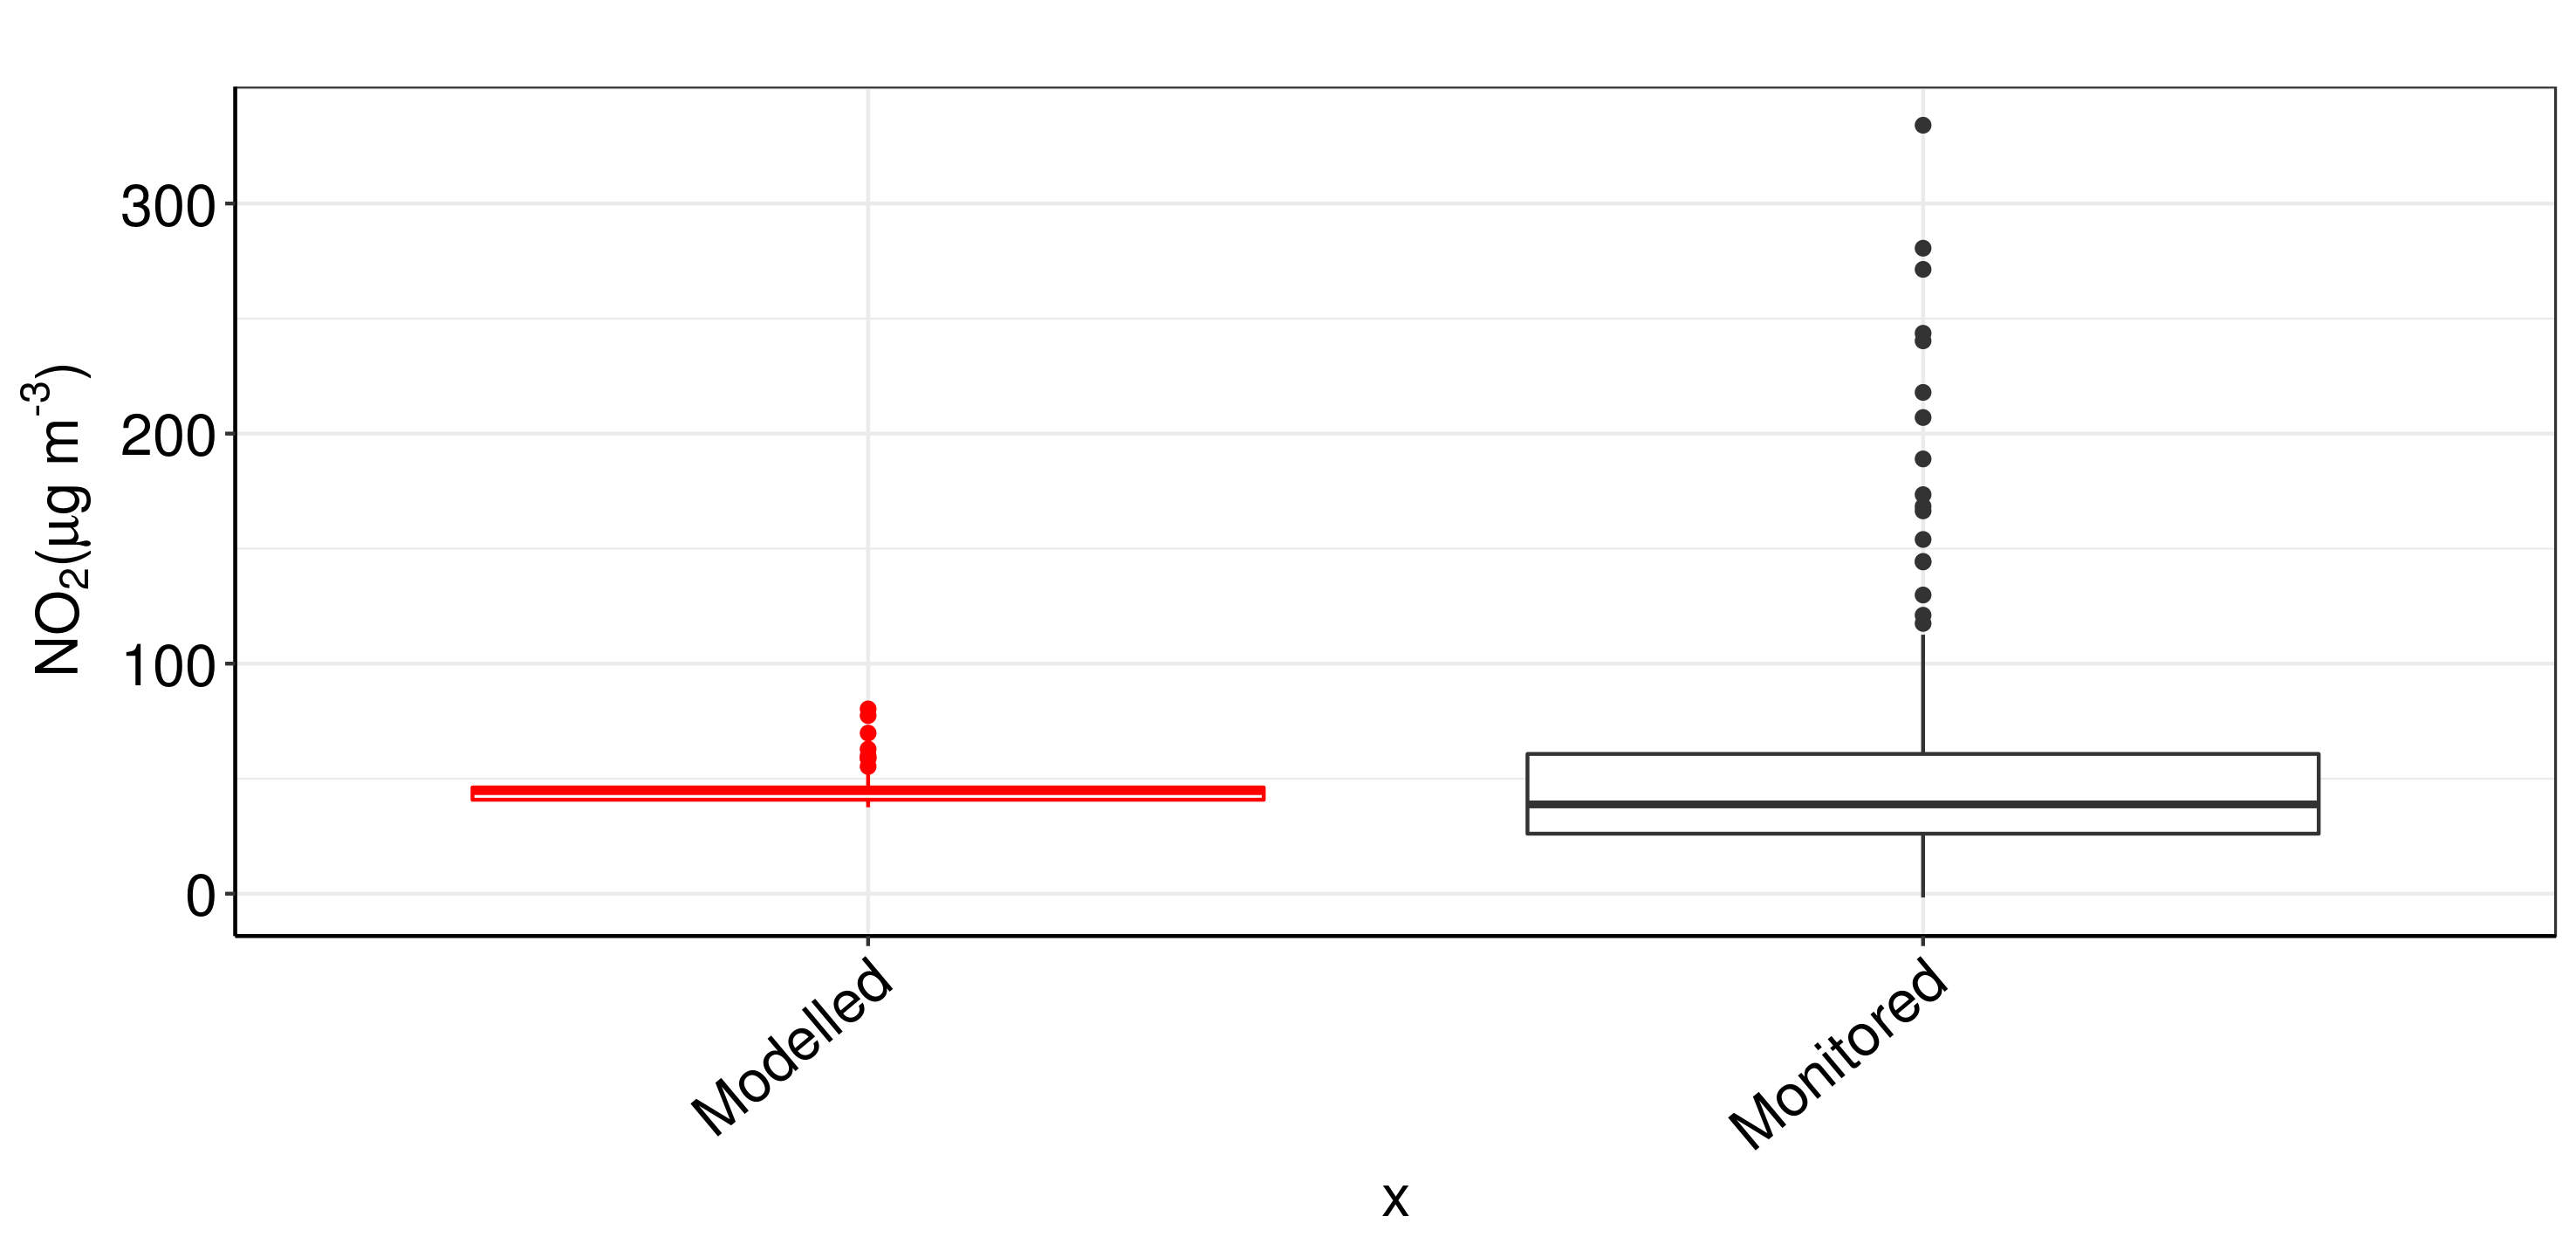
\includegraphics[scale=0.4]{images/grouped_journey_boxplots_new_intercept.png}
%\caption{Boxplot comparison of modelled and monitored concentrations with an intercept of 0 between BC and NO$_{2}$}
%\label{fig:grouped_journey_boxplots_new_intercept}
%\end{figure}

%\begin{figure}[H]
%\centering
%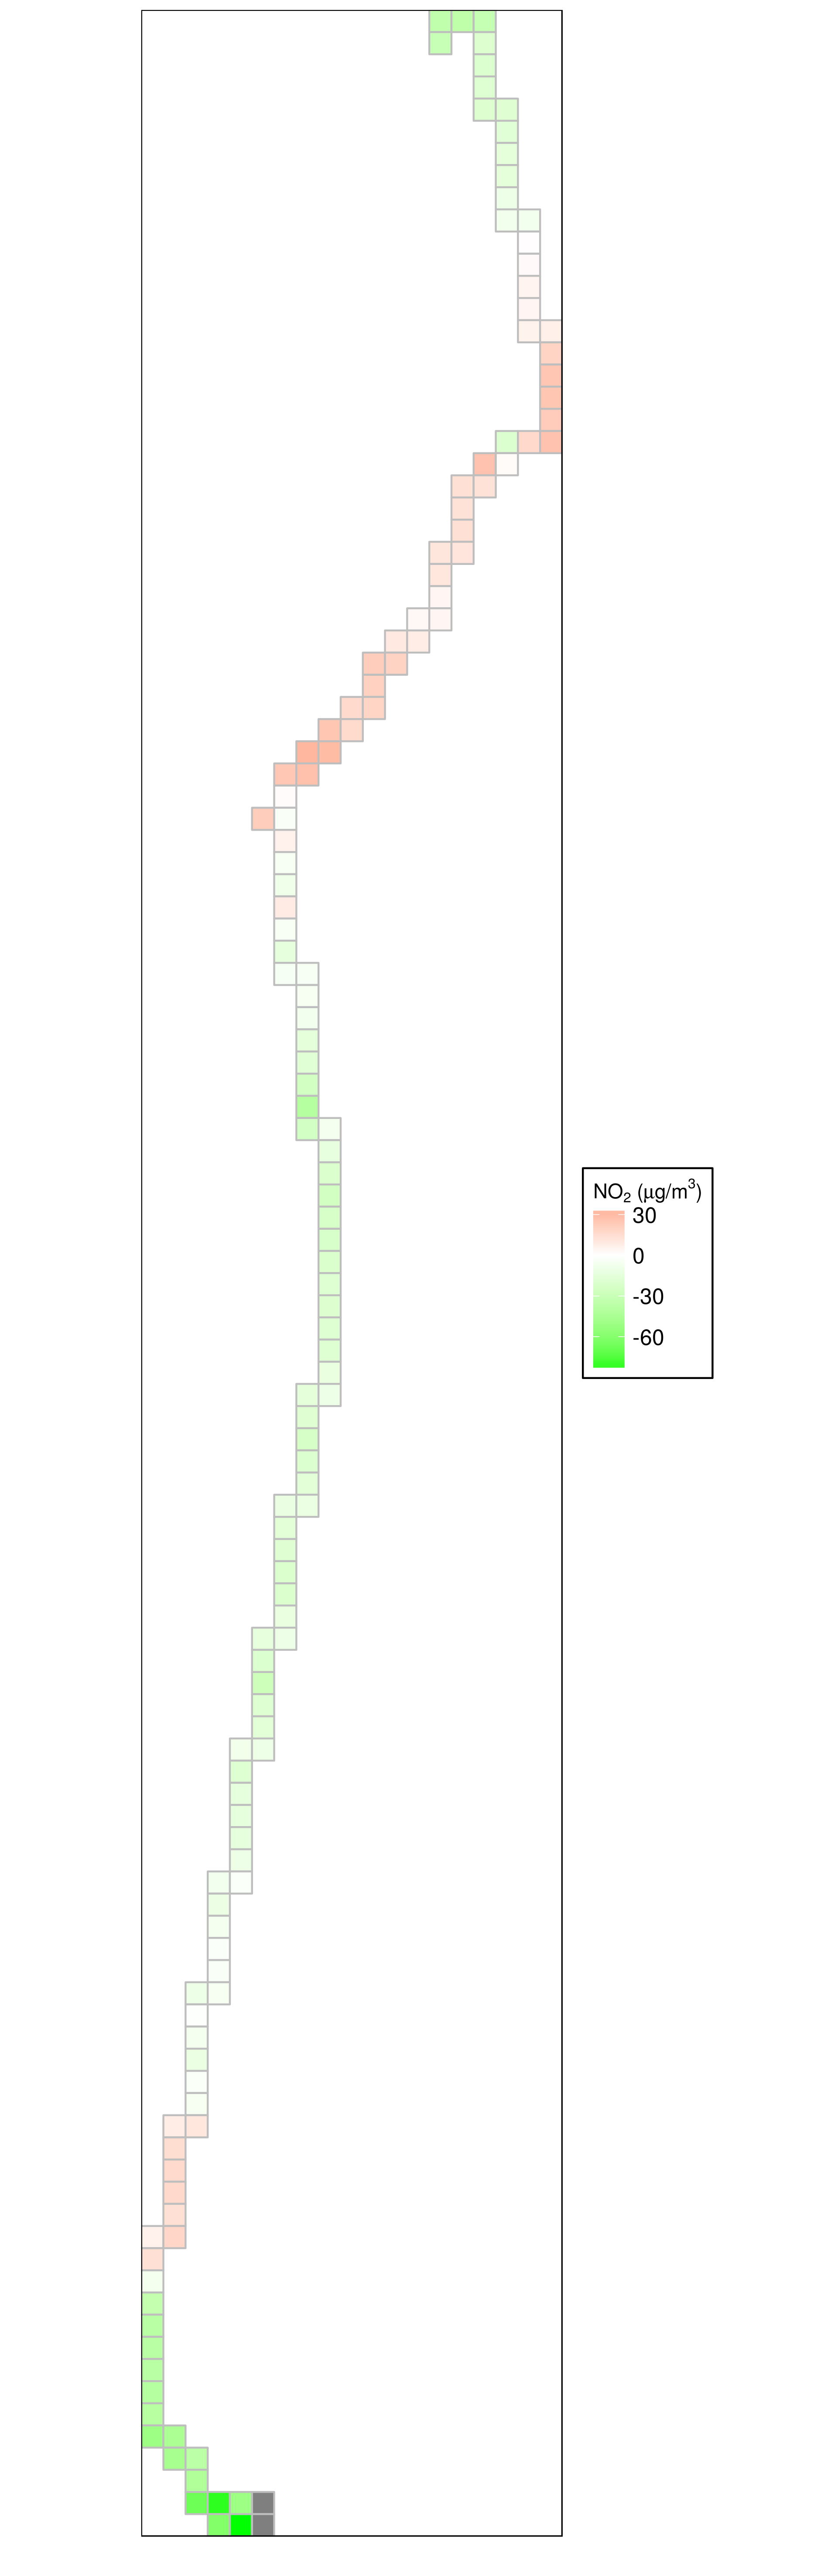
\includegraphics[scale=0.2]{images/monitored_minus_cmaq_route_cells_concs_zero_intercept.png}
%\caption{Spatial comparison of modelled and monitored concentrations with an intercept of 0 between BC and NO$_{2}$}
%\label{fig:monitored_minus_cmaq_route_cells_concs_zero_intercept}
%end{figure}

Putting measurement errors and modelling errors aside, there are practical improvements that could be implemented in repeating this work which might lead to improved results. The most notable being the sample size. If the journey had been shorter, or more researchers were available, it would have been possible to collect a much larger number of samples, which according to the sample size calculations would have increased the reliability of the results. A more practical long-term approach to evaluating air quality model inputs to a hybrid exposure model could be to fix reliable portal monitors to cars or public transport and increase sample size in this manner. For example, mobile monitors might be attached to the outside of a fleet of No.59 buses which run along the route I cycled, meaning each grid square would be sampled 10-15 times between 9am and 10am, resulting in 400-500 measurements over the same time period. Indeed, our group are already trialling a similar method, but with the monitors inside a bus to measure the changes in passenger exposure from the electrification of a bus route in London.

Focusing on the equipment, an unforeseen issue in collecting the monitoring data was a mismatch between cycling speed, the resolution of the CMAQ-UK grid squares, and the temporal resolution of the Microaeth MA300. I wanted to measure concentrations in each grid square along a route, but as the Microaeth was set to 1-minute resolution, the grid squares are 20m by 20m, and typical cycling speed is 15 km/h (or 250 metres per minute), this meant that each minute of Microaeth data covered 250/20 = 12.5 grid squares. Repeating this experiment, a researcher could calculate the sampling rate of the device based upon the likely speed of the movement, and the air quality model resolution it will be compared to, as per equation \ref{eq:sampling_rate_equation}

%\begin{equation}
%  sampling rate_{(minutes)} = \frac{AQ_{(metres)}}{speed_{(metres/minute)}}
%  \label{eq:sampling_rate_equation}
%end{equation}

Though this would of course be constrained by the settings available in the sampling device.

Within the GIS and data processing section of this work, the main issue was the lack of accuracy of the GPS points that were output from the device, how to snap these appropriately to roads (presuming an available roads dataset), and how to link this to CMAQ-UK concentration grid squares for analysis. This was time-consuming and required manual editing at times. Automating this for a large scale campaign would be challenging but necessary. Junctions were a particular difficulty, for instance snapping GPS points at a left-turn always means that the point is snapped to part of the road either side of the junction and never at the actual junction itself (Figure \ref{fig:gps_snapping_error}); which might be where the highest concentrations occur and the researcher is most interested.

%\begin{figure}[H]
%\centering
%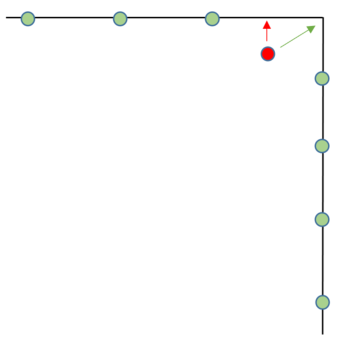
\includegraphics[scale=0.7]{images/gps_snapping_error.png}
%\caption{Accurate GPS points shown in green, GPS error shown in red. Correction should move the point to location shown by green arrow, %but simple ‘snapping’ will move it to direction of red arrow.}
%\label{fig:gps_snapping_error}
%\end{figure}